\section{Résultats}
\subsection{Résultats des évaluations de bcl2fastq et bcl-convert}
\subsubsection{Détermination des meilleurs paramètres pour bcl2fastq}
Après avoir effectué différentes combinaisons des paramètres, il a été mis en évidence que la variation du paramètre \texttt{r} et \texttt{w} en fixant le paramètre \texttt{p}, n'apportait pas de différences significatives pour le temps total d'exécution, le temps cpu ou le pourcentage d'utilisation cpu, comme on peut l'observer sur la figure \ref{barplot-param}, pour p fixé à 12. Des resultats similaires ont été obtenus pour p égale à 4, 8 et 16. 

\begin{figure}[H]
    \centering
    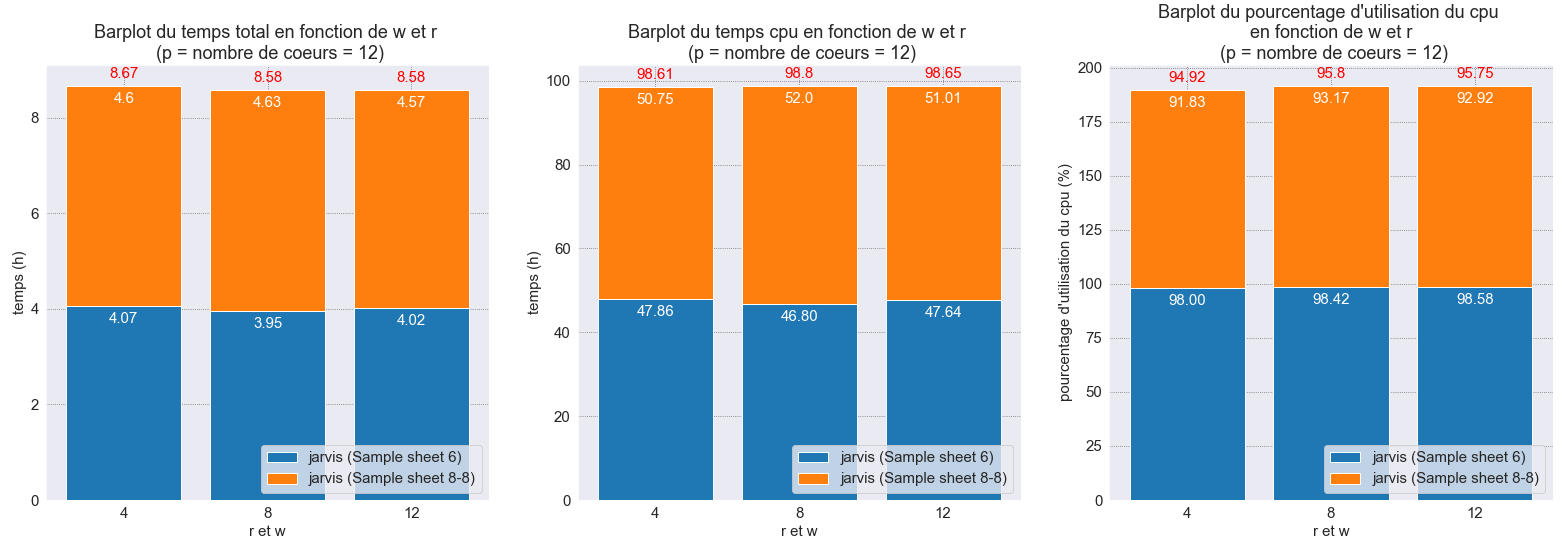
\includegraphics[width=1\textwidth]{img/barplot_cum_jarvis2.png}
    \caption{\footnotesize{Digrammes en bâtons du temps total d'éxécution (à gauche), temps cpu (au milieu) et du pourcentage d'utilisation des cpu (à droite) en fonction des paramètres r et w}}
    \label{barplot-param}
\end{figure}
Il y a deux \emph{sample sheet}\footnote{Fichier contenant les informations et instructions pour la génération des fastq et le démultiplexage}, car le nombre de bases considérés des \emph{reads index} entre les \emph{lanes} est différent, obligeant à réaliser deux appels différents au logiciel pour générer les fastq et le démultiplexage. Ci dessous, la figure \ref{barplot-param2}, représente les résultats obtenus en faisant varier p et en fixant les paramètres r et w à 4 (ces deux paramètres sont fixés à 4 pour pouvoir comparer les 4 résultats). On observe que plus on augmente le nombre de cours et le nombre de \emph{threads} pour p, plus l'execution est rapide. On observe que le temps cpu augmente bien avec le nombre de cœurs et que le pourcentage d'utilisation des cpu est optimal (> 90\%).

\begin{figure}[H]
    \centering
    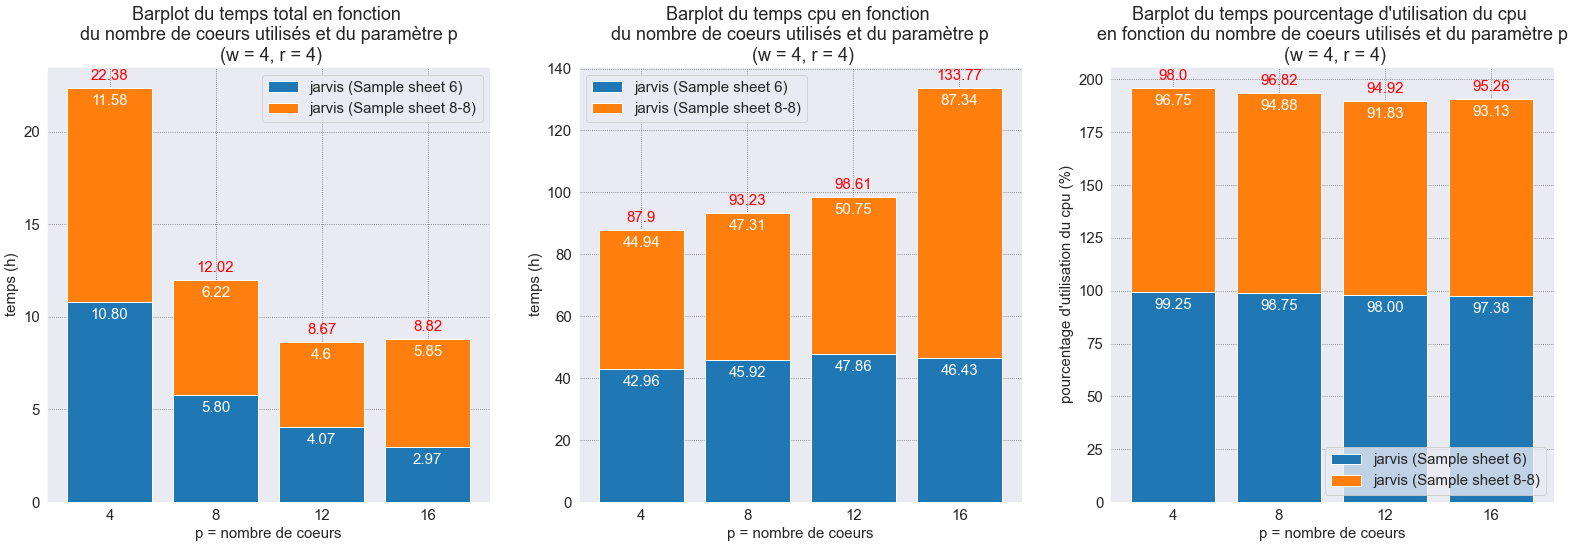
\includegraphics[width=1\textwidth]{img/barplot_cum_jarvis1.png}
    \caption{\footnotesize{Digrammes en bâtons du temps total d'éxécution (à gauche), temps cpu (au milieu) et du pourcentage d'utilisation des cpu (à droite) en fonction du paramètre p}}
    \label{barplot-param2}
\end{figure}

Au vue des résultats obtenus nous avons décidé que les meilleurs paramètres étaient de fixer p à 12, puisque le gain apporté en augmentant à 16 est faible. Néanmoins nous le conserverons pour réaliser la comparaison avec bcl-convert, tout comme p fixé à 8, car il nous permettrait de réaliser deux générations de fastq et de démultiplexage en simultané sur un seul noeud de calcul.\\

\subsubsection{Comparaison entre bcl2fastq et bcl-convert}
J'ai donc fait varier les paramètres \texttt{p}, \texttt{r} et \texttt{w} de manière à ce que chacun des paramètre soient égale au nombre de cœurs accordés aux deux logiciels. On observe bien, sur la figure \ref{fig-total-time}, que plus on augmente le nombre de cœurs pour chacun des logiciels (et donc le nombre de \emph{threads} pour \texttt{p}, \texttt{r} et \texttt{w}) plus la génération des fastq et le démultiplexage est rapide. De plus on remarque que bcl-convert permet de réduire le temps d'environs 1/3 par rapport à bcl2fatq. 

\begin{figure}[H]
    \centering
    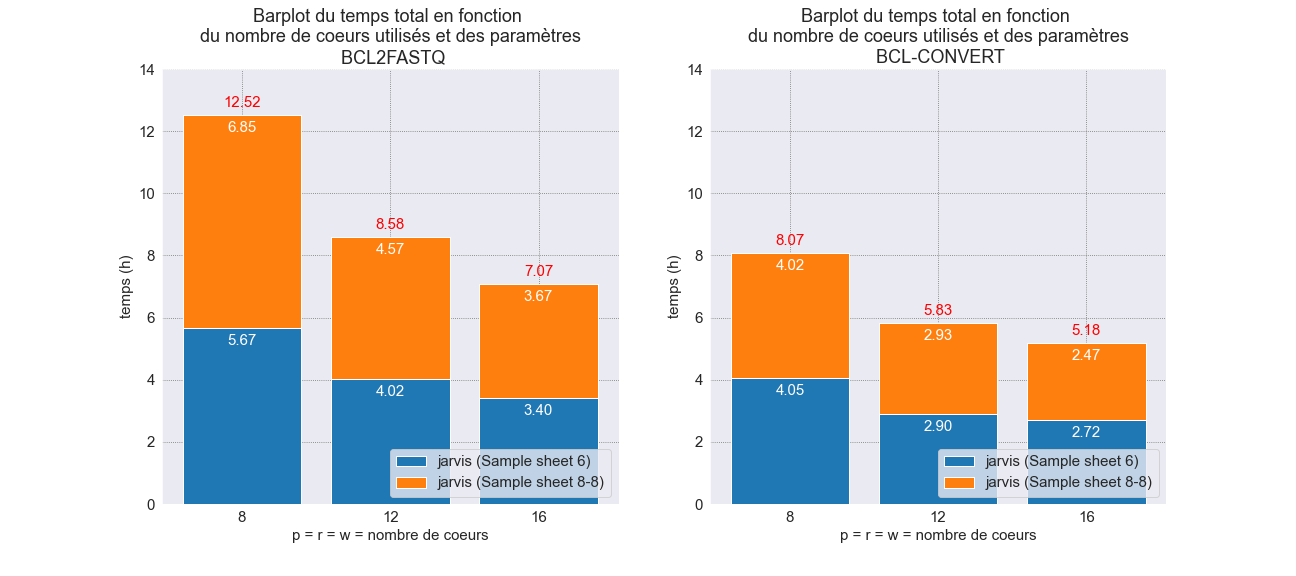
\includegraphics[width=1\textwidth]{img/barplot_total_time_comp.png}
    \caption{\footnotesize{Temps total de génération des fastq pour bcl2fastq et bcl-convert}}
    \label{fig-total-time}
\end{figure}

J'ai également échangé avec le service technique d'Illumina à propos des fichiers de sortie et de l'arborescence de bcl-convert. En effet il s'avère que l'arborescence et les fichiers de sortie sont très différents entre les deux logiciels. Ces échange avaient pour objectif de savoir s'il on pouvait obtenir une arboresnce similaire à bcl2fastq, pour minimiser l'impact du changement de logiciel sur les pipelines. Le changement de bcl2fstq, qui sera bientôt obsolète, par bcl-convert va nous obliger à réaliser de gros changements dans tous les pipelines qui utilisent ces fichiers de sortie et va demander aussi au laboratoire de séquençage de s'adapter à la nouvelle \emph{sample sheet} de bcl-convert.

\subsubsection{Migration de bcl2fastq vers bcl-convert}
Le logiciel bcl-convert étant plus rapide d'environ 1/3 par rapport à bcl2fastq et que ce derniers sera bientôt obsolète. Sachant également, que le nombre de coeurs disponible par noeuds pour la partition \emph{production} du cluster de calcul est de 16 coeurs. Nous avons décidé t'attribuer l'intégralité des coeurs d'un noeud de \og\emph{production} \fg{}, c'est à dire 16 coeurs. L'intégralité des changement entre les deux logiciels à été consignés dans un cahier des charges. Il contient, la commande à lancé pour réaliser le \emph{Base Calling}, modules à charger dans l'environement, le chemin relatif des fichiers de sorties, ainsi qu'un exemple d'arborescence des fichiers de sorties. Ce qui permettera au développeur qui ce chargera de cette migration de suivre ce cahier des charge et ainsi faciliter la migration. Dû à la pression actuelle autour de la technologie MGI, c'est un autre développeur qui sera en charge de réaliser cette migration.


\subsection{Le pipeline NGS\_RG\_MGI}
\textcolor{red}{description des étapes les plus importantes et de l'intéret de les insérer dans NGL.}

\subsection{Le pipeline NGS\_QC\_MGI}
\textcolor{red}{description des étapes les plus importantes et de l'intéret de les insérer dans NGL.}